\begin{frame}{FSEA results}

    \textbf{Details}
    \begin{itemize}
        \item Feature set enrichment analysis on Neuroactive gene sets
        \item Using all kids
        \item Using Mann-Whitney U test
        \item Adjusted q via Benjamini-Hochberg FDR correction
    \end{itemize}
\end{frame}

\begin{frame}{FSEA results}

    \begin{table}
        \tiny
        \begin{tabular}{rrrrrrr}
            \hline\hline
            \textbf{geneset} & \textbf{U} & \textbf{median} & \textbf{mu} & \textbf{sigma} & \textbf{pvalue} & \textbf{qvalue} \\
            \texttt{String} & \texttt{Float64} & \texttt{Float64} & \texttt{Float64} & \texttt{Float64} & \texttt{Float64} & \texttt{Float64} \\\hline
            Menaquinone synthesis & 1.80133e8 & -0.0227514 & -5.3586e7 & 9.71341e6 & 3.45407e-8 & 1.03622e-6 \\
            Propionate degradation & 7.92215e6 & -0.0512878 & -1.02439e7 & 2.70804e6 & 0.0001551 & 0.0023265 \\
            Glutamate degradation & 1.90583e7 & -0.0372657 & -1.24293e7 & 3.56529e6 & 0.000489918 & 0.00489918 \\
            GABA synthesis & 2.3322e7 & -0.029258 & -1.30098e7 & 3.82973e6 & 0.000681137 & 0.00510853 \\
            Tryptophan synthesis & 2.56466e8 & -0.00748907 & -2.68982e7 & 1.06954e7 & 0.0119057 & 0.0605421 \\
            SAM synthesis & 6.56769e7 & -0.0162254 & -1.42519e7 & 5.68037e6 & 0.0121084 & 0.0605421 \\
            p-Cresol synthesis & 3.26506e7 & -0.0350193 & -8.52534e6 & 4.07706e6 & 0.0365233 & 0.148674 \\
            Acetate synthesis & 2.16053e8 & -0.0120984 & -2.00878e7 & 9.7636e6 & 0.0396464 & 0.148674 \\
            Quinolinic acid degradation & 1.48097e8 & -0.0162254 & -1.53888e7 & 8.12391e6 & 0.058191 & 0.193307 \\
            Butyrate synthesis & 4.47099e7 & -0.0306039 & -8.57642e6 & 4.63802e6 & 0.0644355 & 0.193307 \\\hline\hline
        \end{tabular}
    \end{table}

\end{frame} 

\begin{frame}{Menaquinone synthesis}
    \begin{columns}[c] % The "c" option specifies centered vertical alignment while the "t" option is used for top vertical alignment

        \column{.7\textwidth} % Right column and width
        \begin{figure}
            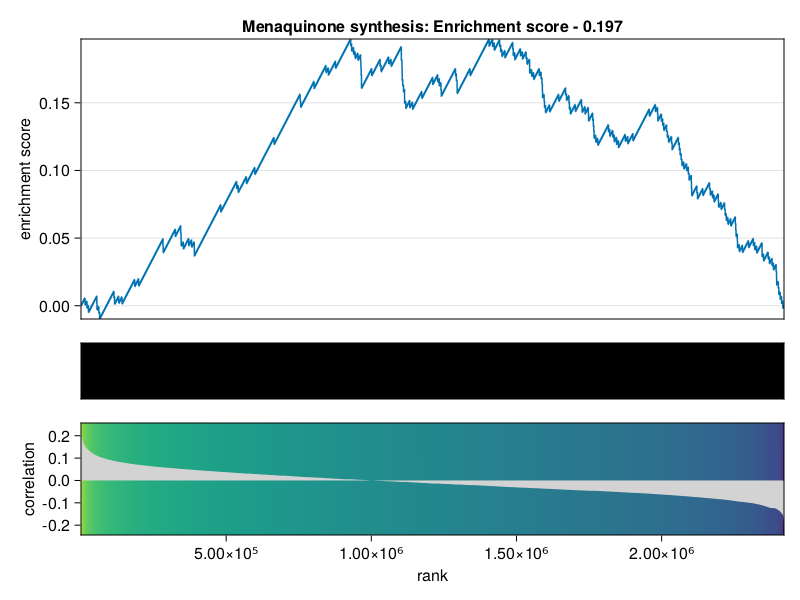
\includegraphics[width=1\linewidth]{../figures/fsea_Menaquinone-synthesis.png}
        \end{figure}

    \end{columns}

\end{frame}

\begin{frame}{Propionate degradation}
    \begin{columns}[c] % The "c" option specifies centered vertical alignment while the "t" option is used for top vertical alignment

        \column{.7\textwidth} % Right column and width
        \begin{figure}
            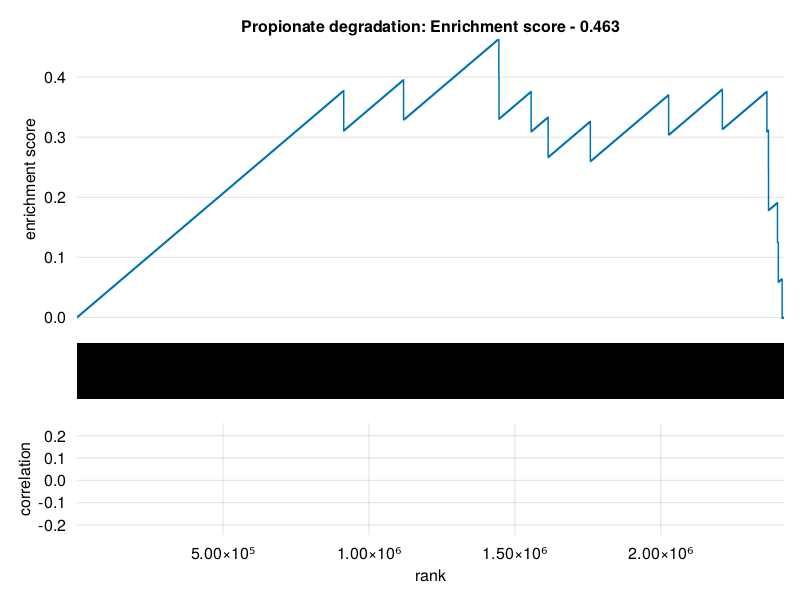
\includegraphics[width=1\linewidth]{../figures/fsea_Propionate-degradation.png}
        \end{figure}

    \end{columns}

\end{frame}

\begin{frame}{Glutamate degradation}
    \begin{columns}[c] % The "c" option specifies centered vertical alignment while the "t" option is used for top vertical alignment

        \column{.7\textwidth} % Right column and width
        \begin{figure}
            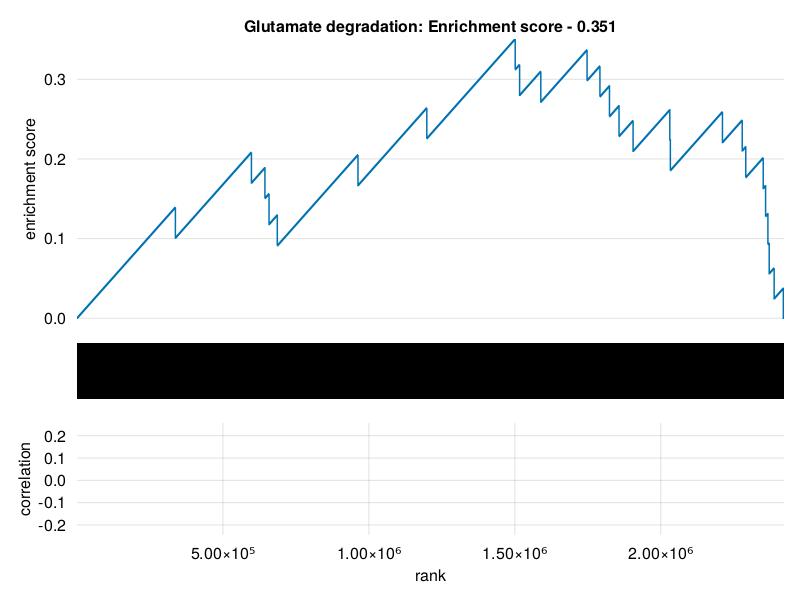
\includegraphics[width=1\linewidth]{../figures/fsea_Glutamate-degradation.png}
        \end{figure}

    \end{columns}

\end{frame}

\begin{frame}{GABA synthesis}
    \begin{columns}[c] % The "c" option specifies centered vertical alignment while the "t" option is used for top vertical alignment

        \column{.7\textwidth} % Right column and width
        \begin{figure}
            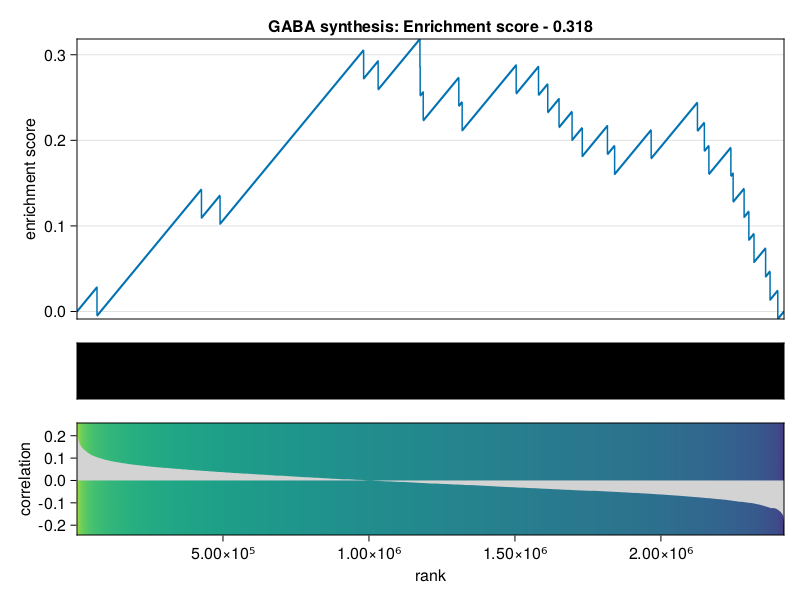
\includegraphics[width=1\linewidth]{../figures/fsea_GABA-synthesis.png}
        \end{figure}

    \end{columns}

\end{frame}

\begin{frame}{Tryptophan synthesis}
    \begin{columns}[c] % The "c" option specifies centered vertical alignment while the "t" option is used for top vertical alignment

        \column{.7\textwidth} % Right column and width
        \begin{figure}
            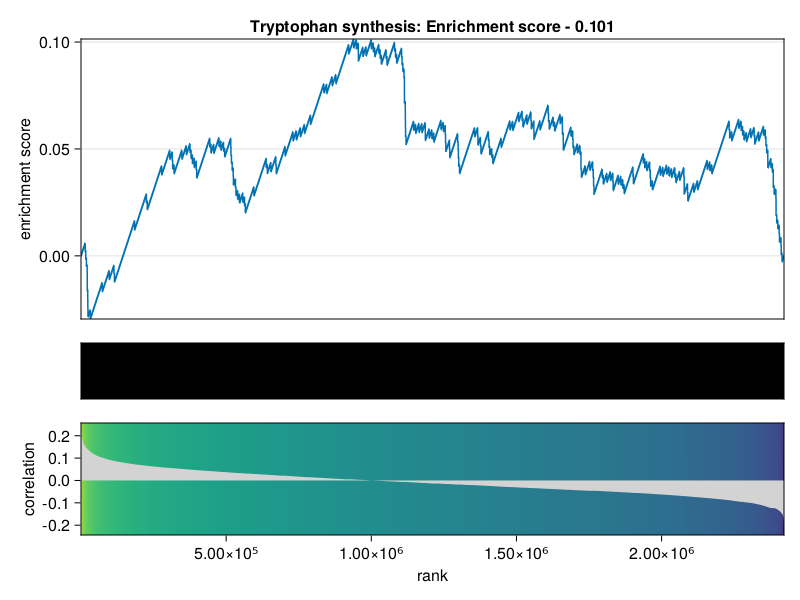
\includegraphics[width=1\linewidth]{../figures/fsea_Tryptophan-synthesis.png}
        \end{figure}

    \end{columns}

\end{frame}

\begin{frame}{SAM synthesis}
    \begin{columns}[c] % The "c" option specifies centered vertical alignment while the "t" option is used for top vertical alignment

        \column{.7\textwidth} % Right column and width
        \begin{figure}
            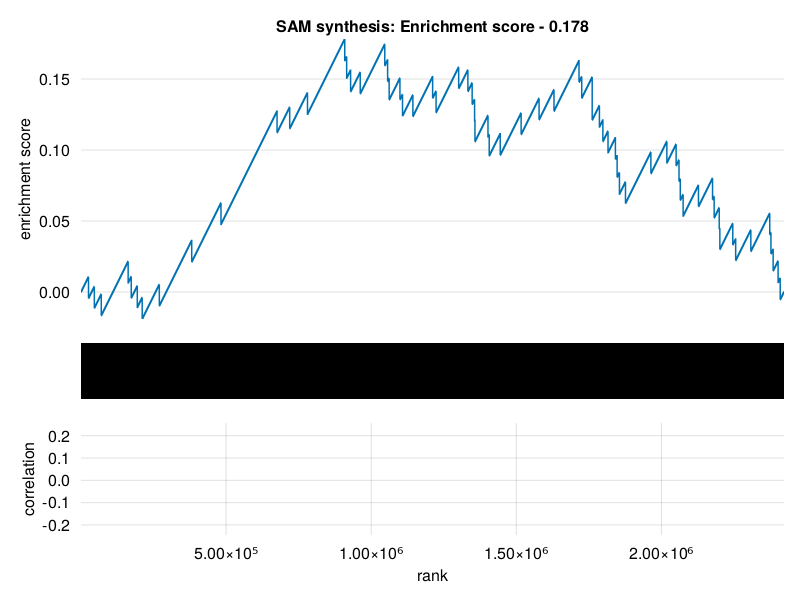
\includegraphics[width=1\linewidth]{../figures/fsea_SAM-synthesis.png}
        \end{figure}

    \end{columns}

\end{frame}

\begin{frame}{p-Cresol synthesis}
    \begin{columns}[c] % The "c" option specifies centered vertical alignment while the "t" option is used for top vertical alignment

        \column{.7\textwidth} % Right column and width
        \begin{figure}
            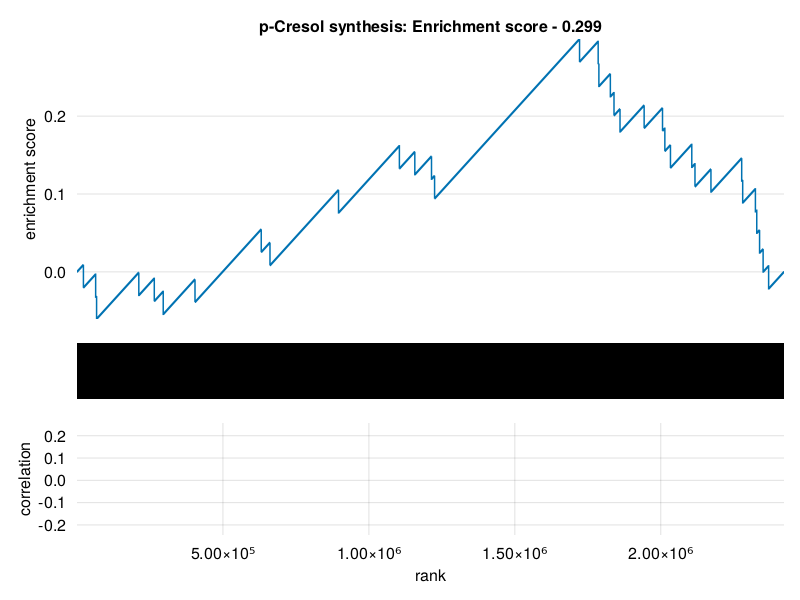
\includegraphics[width=1\linewidth]{../figures/fsea_p-Cresol-synthesis.png}
        \end{figure}

    \end{columns}

\end{frame}

\begin{frame}{Acetate synthesis}
    \begin{columns}[c] % The "c" option specifies centered vertical alignment while the "t" option is used for top vertical alignment

        \column{.7\textwidth} % Right column and width
        \begin{figure}
            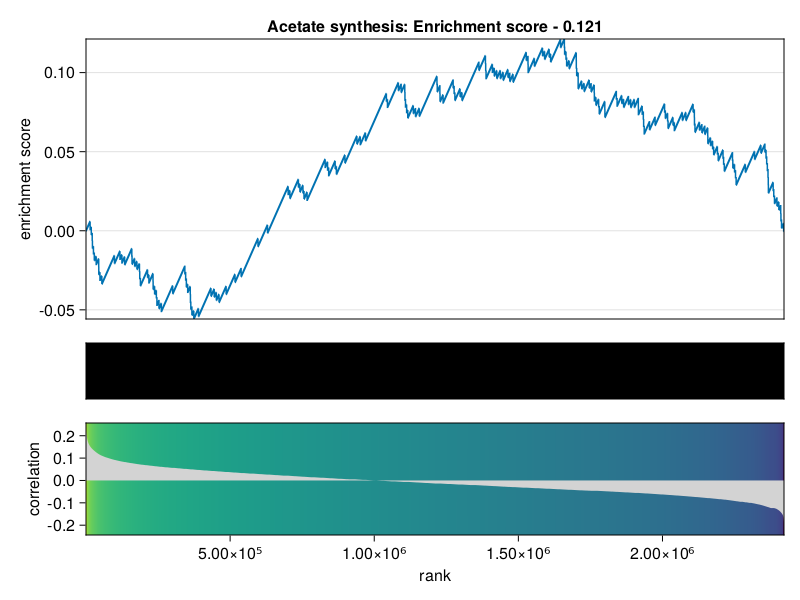
\includegraphics[width=1\linewidth]{../figures/fsea_Acetate-synthesis.png}
        \end{figure}

    \end{columns}

\end{frame}

\begin{frame}{Quinolinic acid degradation}
    \begin{columns}[c] % The "c" option specifies centered vertical alignment while the "t" option is used for top vertical alignment

        \column{.7\textwidth} % Right column and width
        \begin{figure}
            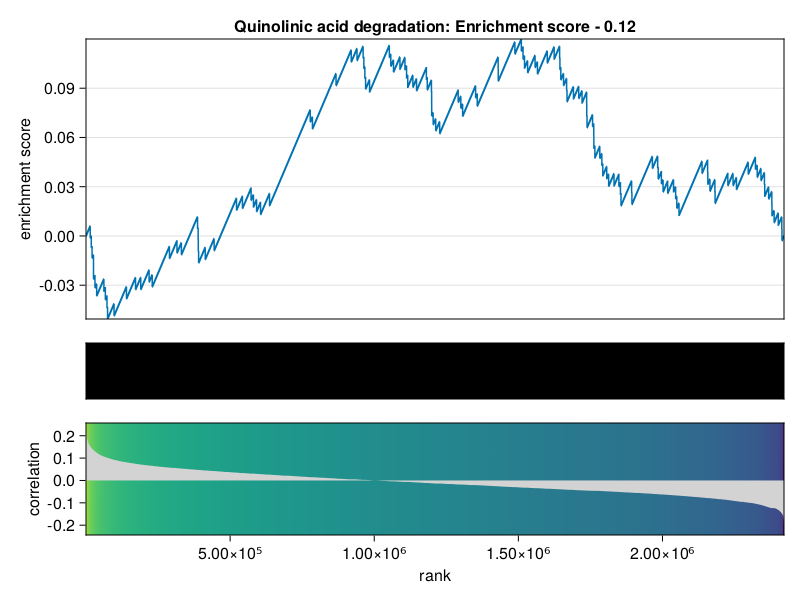
\includegraphics[width=1\linewidth]{../figures/fsea_Quinolinic-acid-degradation.png}
        \end{figure}

    \end{columns}

\end{frame}

\begin{frame}{Butyrate synthesis}
    \begin{columns}[c] % The "c" option specifies centered vertical alignment while the "t" option is used for top vertical alignment

        \column{.7\textwidth} % Right column and width
        \begin{figure}
            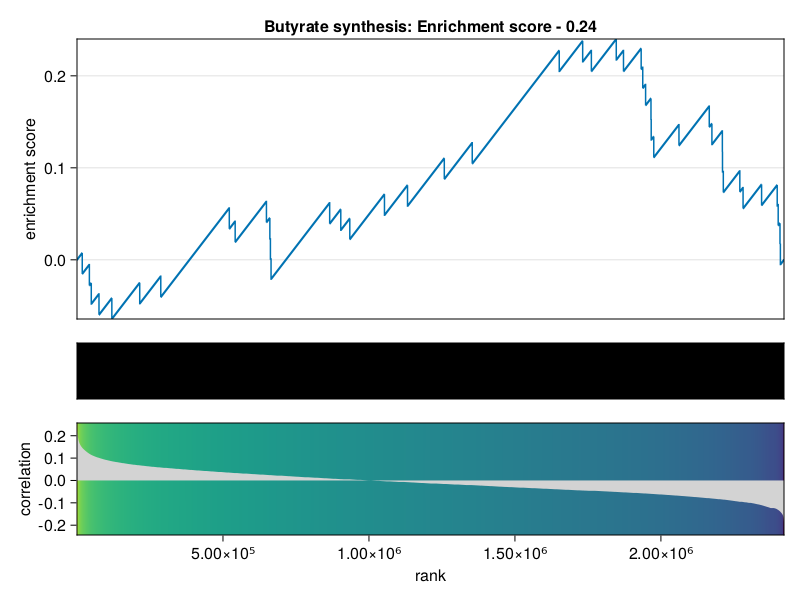
\includegraphics[width=1\linewidth]{../figures/fsea_Butyrate-synthesis.png}
        \end{figure}

    \end{columns}

\end{frame}
